%!TEX TS-program = xelatex
%!TEX encoding = UTF-8 Unicode

\documentclass{../Dissertate}
%% \documentclass{../DissertatePrint}
%% \usepackage{comment}
%% \excludecomment{figure}
%% \let\endfigure\relax

\begin{document}

\doublespacing

\setcounter{chapter}{5}
\chapter{Intuition vs. Reflection in Reasoning}

\section{Introduction}

In Chapter 3, we saw that 
induction can be driven by more than one kind of information,
as perceptual similarity and conceptual knowledge
came into conflict during reasoning.
\citet{Bright2014a}, in their hybrid theory,
proposed a more subtle distinction in inductive reasoning,
between associative and structured knowledge.
While a number of results show that both kinds of knowledge
can drive inductive reasoning, however,
less is known about how these kinds of knowledge interact.
This is the question I seek to answer in this chapter.

As \citet{Bright2014a} note,
theories of induction can be classed in two ways.
Some theories propose that induction is based on structured knowledge:
the world is organised into coherent categories,
and specific knowledge about these categories,
and the often complex relationships between them,
is used as the basis for inference.
One such theory is \citegap{Osherson1990}{'s} similarity coverage model,
that describes inferences about species of animal
with reference to the taxonomic relationships between them.
More recent accounts have generalised this idea,
casting induction as a process of Bayesian inference
\citep{Griffiths2009,Griffiths2005,Heit1998,Kemp2009}.
At the core of these accounts is the notion that
in category-based induction,
we attempt to use the information given in the premises
(i.e. ``Carrots have disease X'')
to update our beliefs about the distribution of this property
across all categories.
To do so, we must be able to express how various categories are related:
the probability that rabbits have a given disease, given that carrots have it,
depends on the means by which diseases can be transmitted between various species,
in this case, through ecological interactions, such as a food chain.
Similarly, biological properties, such as genes,
are most strongly projected according to 
the distance between species in the taxonomic tree \citep{Heit1998,Osherson1990},
while if we know that certain artefacts are found in one city,
geographical distance is used to decide which other cities are likely to
house them \citep{Kemp2009}.

On the other hand,
a number of theories of inductive inference,
and category-based induction in particular,
rely on simpler, \emph{associative} forms of knowledge.
Similarity, including visual similarity,
discussed in Chapter 3, is one such form of knowledge;
things that are similar
\citep[share many properties, or features, that we know of; see][]{Medin1993}
are likely to also share novel properties.
For instance, on learning about two animals, both of which
live underwater, have scales, and breathe through gills,
we do not need to know what a ``fish'' is
to predict that if one lays eggs, the other likely does as well.
Of course, as discussed in Chapter 3, similarity comes in many forms,
and \citet{Fisher2015} make a useful distinction between
perceptual and representational (i.e. knowledge-based) similarity.
Perceptual similarity is most often proposed
as the basis of induction in children
\citep[][see also Chapter 3]{Sloutsky2010,Sloutsky2008,Sloutsky2007}.
A number of theories of induction in adults,
however, are based on the overlap of features
in our mental representations \citep{Rogers2004,Rogers2008,Sloman1993}
or perceptual input \citep{Sloutsky2008,Sloutsky2004}.
Other associative accounts of induction,
including of inductive generalisation during learning, are based on
what is variously referred to as contiguity, co-occurrence, or thematic relations:
things that are often seen together are more likely 
to share properties than things that are not
\citep{Kruschke1992,Rumelhart1986,Rescorla1972}.

% Also cited:
% Colunga & Smith, 2005;
% French, Mareschal, Mermillod, & Quinn, 2004; Jones & Smith, 2002; Sloutsky, Kloos, &
% Fisher, 2007).
% Smith and DeCoster (2000)

\citet{Bright2014a} argue that neither
structured nor associative accounts of induction alone are complete.
As noted by \citet{Murphy1985},
associative accounts of categorisation and induction
fail to capture some of the flexibility and complexity seen in human reasoning.
In particular, participants have been shown to be
sensitive to property effects when reasoning inductively:
the strength of an argument is dependent
on the kind of property projected
\citep{Heit1994,Shafto2007,Shafto2005}.
Therefore, transmittable properties such as infectious diseases
are thought to be shared by animals that are related ecologically,
such as predators and prey in a food chain,
whereas biological properties such as genes are shared 
only by animals that are close together in their taxonomic tree.
It is difficult to account for such flexibility in a purely associative account
\citep[but see work by][]{Sloutsky2008,Rogers2004}.
Structured models such as the Bayesian accounts discussed above \citep[i.e.][]{Kemp2009},
in contrast, draw on different knowledge structures for different inferences,
and so can capture this flexibility in human reasoning.

At the same time, it seems unlikely that 
structured knowledge alone drives inductive reasoning.
Induction is an ubiquitous phenomena, encompassing any inference that goes
``beyond the information given'' \citep{Bruner1973}.
This ranges from simple perceptual inferences,
to the development and postulation of scientific theories
\citep[see][for a taxonomy of inductive inferences]{Kemp2014}.
Furthermore, inductive reasoning is not exclusive to human adults:
similar inferences, although in simpler domains,
must be made both by children, and throughout the animal kingdom.
Associative theories of induction provide accounts that
make more reasonable claims about the cognitive abilities
required to reason inductively.
Indeed, in the spirit of \citet{Simon1956},
associative processes may \emph{satisfice},
often yielding the same inferences as structured accounts,
but with considerably less effort.

Faced with this dichotomy between associative and structured knowledge in induction,
\citet{Bright2014a} proposed a theory that combines both forms of knowledge.
This \emph{hybrid} theory claims
that both kinds of knowledge are drawn upon during reasoning,
with a key distinction between the two being their processing characteristics.
By this account, associative knowledge can be retrieved quickly and easily,
while structured knowledge is slower to retrieve,
and places greater demands on working memory to utilise.

Evidence for this hybrid theory
comes from experiments that manipulate 
the processing conditions under which participants reason.
This research is discussed in more detail in Chapter 1, but to recapitulate,
participants' inferences (their choices, or ratings of argument strength)
are predicted by measures of associative knowledge under all circumstances.
Furthermore, under favourable conditions only
(i.e. in the absence of time pressure, or cognitive load),
inferences are additionally predicted by
appropriate measures of structured knowledge,
such as whether participants believed two species
belonged to the same taxonomic group
when reasoning about biological properties.

Of particular relevance to this thesis, which focuses on \emph{conflict} in reasoning,
\citeauthor{Bright} (\citeyear{Bright}, see also \citealp[Chapter 5]{Crisp-Bright2010})
report a version of the inductive triad task \citep{Gelman1986}
that places associative and structured knowledge directly in conflict.
In the trial shown in Figure~\ref{fig:crisp_screenshot}, for example,
participants were told a biological property of carrots (they have ``C5s cells''),
and chose between generalising this property to rabbits, or to bamboo.
Carrots and rabbits are strongly associated,
and so a participant relying on associative knowledge
would project a property from carrots to rabbits.
This is despite the fact that the link between the species is a food chain,
and so doesn't provide a means for them to share a biological property.
Carrots and bamboo, on the other hand, are both plants,
and so are more likely to share such a property.
The associative link between the two species, however,
is substantially weaker, and so projecting the property to bamboo
requires that one inhibits the associative knowledge linking carrots and rabbits
before one can draw on the structured link between carrots and bamboo instead.
Consistent with the hybrid theory,
participants were less likely to select the
taxonomically-related response option
over a strongly associated foil in this task
when under heavy cognitive load,
or if they had poor semantic inhibitory control
\citep[a measure of their ability to inhibit
  task-irrelevant semantic information;][]{Markovits2004,Burgess1996a}.
Like most studies that analyse only participants' ultimate responses, however,
while these results do reveal what information drove participants' final choices,
we are limited in what conclusions we can draw about
how different processes interact during this task.
To address this shortcoming, in this chapter I present
a mouse tracking extension of the \citet{Bright} triad task.

\begin{figure}[ht]
  \centering
  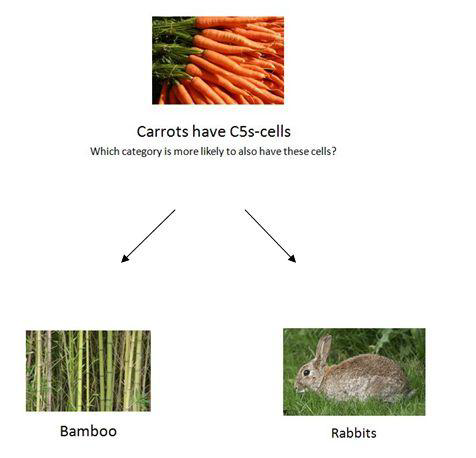
\includegraphics[width=\figurewidth]{imgs/crisp_screenshot.png}
  \caption[A conflict trial from \citet{Bright}.]{
    A conflict trial from \citet{Bright}.
    Participants learn that carrots posses the given biological property,
    and asked which of the other two species, bamboo or rabbits,
    are likely to share this property.
    \label{fig:crisp_screenshot} }
\end{figure}


How might associative and structured knowledge interact during this task?
Again, I propose two possibilities.
First, it may be that people selectively draw on associative knowledge
\emph{or} structured knowledge for a given inference.
In this case, we would expect to find
little evidence of actual conflict during reasoning,
as both kinds of knowledge would not compete during a single trial.
This would lead to cursor trajectories where
participants move directly towards one or other option, and then select it,
rather than changing direction mid-flight.
The second possibility is that
associative knowledge may be activated early in reasoning,
but be later overridden, at least some of the time,
by slowly-retrieved, more cognitively demanding structured knowledge.
In this case, participants would be conflicted
when they do override, or at least attempt to override,
their association-driven response.
Cursor trajectories in this case should largely be
initially drawn to the foil species
when it is cued by associative knowledge,
but also likely to override this initial movement
and select the correct species instead
at least some of the time.






\section{Method}

\subsection{Participants}

One hundred and thirty one students at Queen’s University Belfast
participated in exchange for course credit.

\subsection{Materials}

Eight problems were adapted from
\citegap{Primi2015}{'s} extended version of the CRT.
Each of these problems was modified to create a set of
eight corresponding non-conflict problems,
in which the intuitively appealing responses were also the correct ones
(see the Appendix~\ref{appendix:exp6_stimuli}).
Participants were randomly allocated to complete either
conflict versions of items 1, 3, 5, and 7
and no-conflict versions of the rest, or vice versa.
Each problem was presented in a 4-option multiple choice format.
For the conflict items, the possible responses were the correct option,
the incorrect heuristic option, and two incorrect foil options.
For the non-conflict items the correct intuitive option was presented
with three incorrect foils.

\subsection{Procedure}

The experiment was administered on personal computers,
programmed using PsychScript (see Chapter 2),
and run in the web browser.
Participants were instructed to respond in their own time to each CRT problem
by clicking on one of the four response options
presented in the four corners of the display
(Figure~\ref{fig:exp6-screenshot}).
Participants were not made aware of
the mouse tracking aspect of the experiment in advance. 

\begin{figure}[ht]
  \centering
  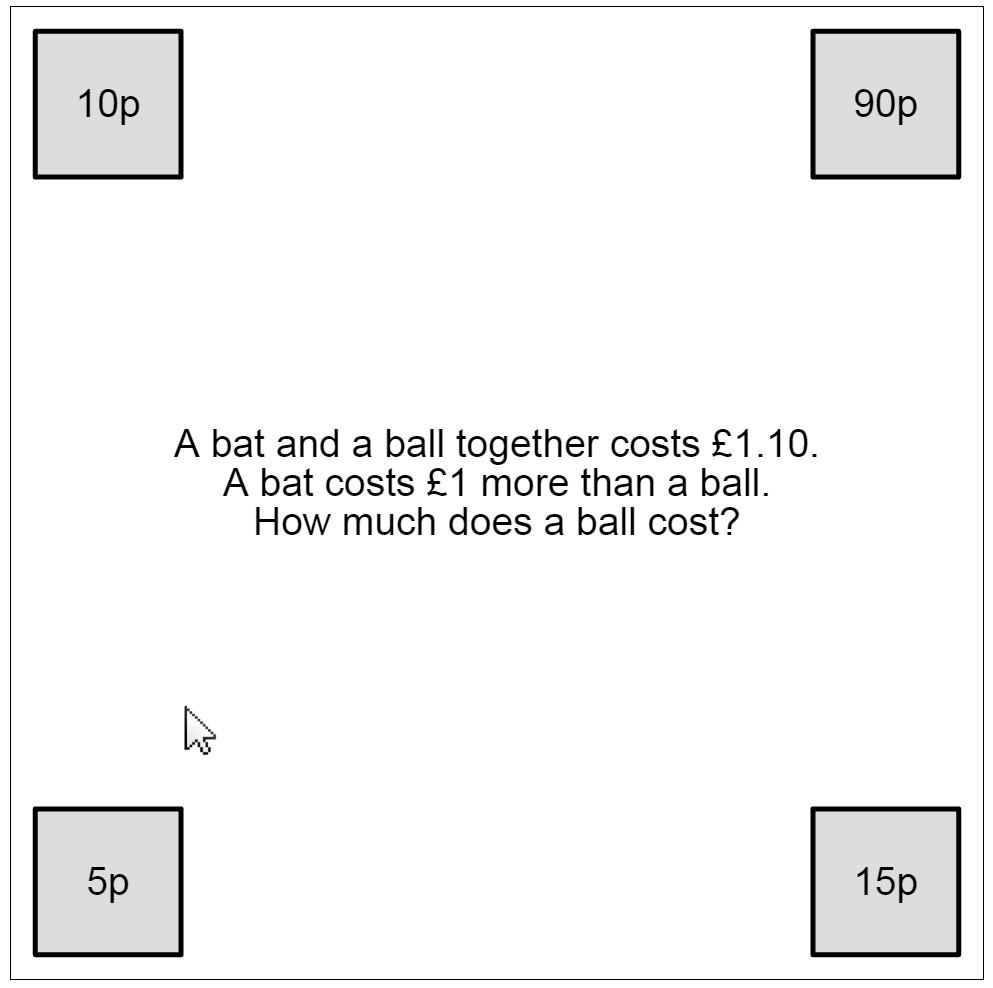
\includegraphics[width=\figurewidth]{imgs/exp6-screenshot.png}
  \caption[A screen shot from the CRT, Experiment 6.]{
    \label{fig:exp6-screenshot}
    A screen shot from the CRT.
  }
\end{figure}

Each problem was preceded by onscreen instructions to
click on a button marked ``Go'', presented in the centre of the monitor.
This was done to ensure the mouse cursor was located
in the same central position at the beginning of each trial.
The button was then replaced by the problem text
and the four response options appeared simultaneously in the corners
(Figure~\ref{fig:exp6-screenshot}).
The response options were randomly assigned to the four locations on each trial,
with the constraint that the correct and heuristic response options
were always adjacent for conflict problems.
The mouse cursor was no longer visible at the onset of each trial
to prevent it from obscuring the question text.
The cursor reappeared once it had been moved more than 5\% of the width of the display.
Mouse cursor location was recorded every 20 msec.


\section{Results}

\subsection{By-trial analyses}

After excluding data from 3 participants 
who did not complete the experiment within the 15 minutes allocated, 
and 7 trials with response times greater than 100 seconds (.6\% of the total), 
participants selected the correct option on 79.5\% of non-conflict problems.
On the conflict problems, the correct option was chosen 36\% of the time,
the heuristic option 58\%, and one of the foils 6\% of the time.

In the first stage of the analysis, 
I calculate a number of summary statistics for each trial, 
and compare these between problem types, and between responses. 
The measures were response time, 
the distance travelled by the mouse cursor
(scaled so that a straight line from the start point
 to the response corresponds to 1 unit),
the number of times the cursor was moved during a trial
(with movements defined as windows of 100 msec or more in motion, 
separated by 100 msec or more not moving), 
the closest proximity achieved between 
the cursor and the non-chosen option
(closest proximity to the heuristic response option 
on trials where the correct option was chosen, and vice versa). 
These measures were compared using linear mixed models, 
with crossed random intercepts for each participant, 
and each problem \citep{Baayen2008}.
Response latencies, and the distance travelled by the mouse cursor
were log-transformed to normalise their distributions, 
and a generalised mixed model with a Poisson link was used
to model the number of movements. 

Consistent with a dual process interpretation, 
whereby heuristic responses are generated by Type 1 processes,
and correct responses under conflict by Type 2 processes,
for conflict problems there was greater evidence of conflict
across all measures when participants gave the correct response (N = 181) 
than the heuristic one (N = 297).
The average time to respond was 27.3 seconds (SD = 16.3) for correct responses, 
and 21.0 seconds (SD = 13.4) for heuristic responses
($e^{\beta}$ = 114\%, CI = [102\%, 129\%],
t(470.8) = 2.349, p = .0192).
The mouse cursor travelled a greater distance 
before selecting a correct option (6.11 times the minimum needed distance, SD = 5.6) 
than an heuristic option (5.66 times, SD = 4.74;
$e^{\beta}$ = 116\%, CI = [102\%, 133\%],
t(298.4) = 2.267, p = .0241). 
There were also more cursor movements on
trials in which the correct response was given (5.4, SD = 4.8) 
than when the heuristic response was given (4.9, SD = 4.5; 
$e^{\beta}$ = 1.15, CI = [1.02, 1.29],
z = 2.337, p = .0195).
Finally, the minimum distance between 
the cursor and the heuristic option on trials in which the correct option was chosen 
was on average 49\% of the display width (SD = 24\%),
significantly less than the minimum distance between
the cursor and the correct option 
on trials in which the intuitive option was chosen (55.5\%, SD = 18\%,
$e^{\beta}$ = 0.92, CI = [0.89, 0.96],
t(72.1) = 4.119, p < .0001).

Most tests of the intuitive logic model compare
correct responses on no-conflict problems with
heuristic responses on conflict problems, 
on the basis that heuristic, Type 1 processes should cue both kinds of response, 
but the chosen response conflicts with normative principles on conflict problems only. 
Evidence for the intuitive logic model 
therefore comes from results which indicate 
greater conflict for heuristic responses to conflict problems (N = 404). 
However, there was no such reduction in conflict for no-conflict problems
on any of the applicable measures:
response time (23.1 seconds, SD = 15.3; t(14.3) = 0.222, p > .8),
distance travelled (5.6, SD = 5.0; t(15.0) = 0.359, p > .7) 
and number of movements per trial (5.2, SD = 4.6; z = 0.064, p > .95).

Following previous intuitive logic studies
\citep[e.g.][see also \citealp{Pennycook2015}]{DeNeys2011b,Mevel2014},
I also calculated the number of heuristic responses given
by each participant on conflict problems, 
and categorised each participant as either
``majority heuristic'' (3 or 4 heuristic responses out of four, 53 participants)
or ``minority heuristic'' (0 to 2 heuristic responses, 75 participants). 
I entered this measure as a participant-level predictor in the models, 
but found that it was not involved with any interactions in the analyses above
(t's < .9, p's > .4). 
I also repeated this analyses for the most (4 heuristic responses) 
and least (one heuristic response) biased reasoners only, 
again finding so significant interactions (t's < 1.1, p's > .25).
Therefore, these analyses revealed no evidence for logical intuitions
in either biased or unbiased participants.



\subsection{Time Course Analyses}

\begin{figure}[ht]
  \centering
  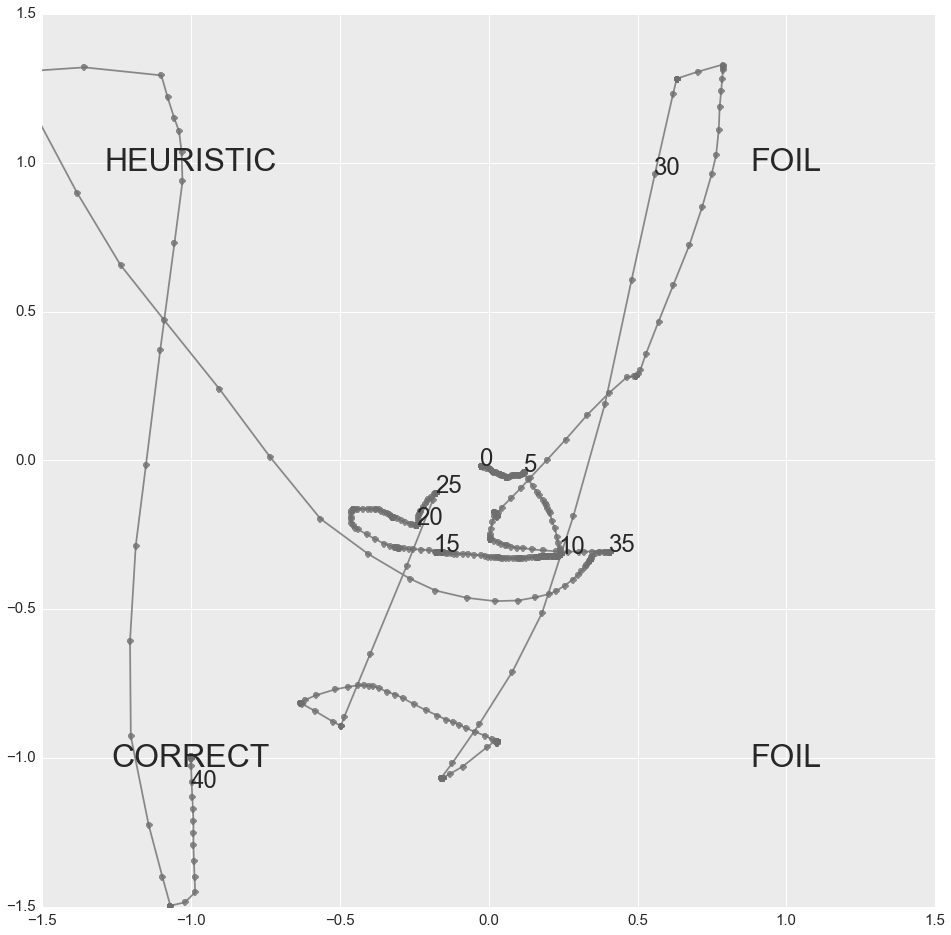
\includegraphics[width=\figurewidth]{imgs/exp6-typical-trajectory.png}
  \caption[A typical cursor trajectory from Experiment 6.]{
    \label{fig:exp6-typical-trajectory}
    A typical mouse cursor trajectory from the conflict condition. 
    Numerical values indicate the time elapsed in seconds. 
    Cursors meandered as participants generated their responses, 
    passing near the response options located in the corners of the display
  }
\end{figure}

In most previous mouse tracking research,
both in this thesis and in general
\citep[e.g.][]{Freeman2011d,Spivey2005},
the location of the cursor is recorded over a few seconds,
as participants move it from a starting position to 
a response option located in either top corner of the screen.
Almost invariably, this path follows either a single movement
(curved or otherwise) to a response,
or as has been more the case in this thesis,
a movement towards one response, that changes direction mid-flight.
In the current data, unfolding over up to 60 seconds, 
participants move and rest the cursor many times throughout a trial,
an average of 5.1 times, and a maximum of 30.
Thus, this data is in ways more similar to eye movement data.
A typical mouse cursor trajectory is shown in Figure~\ref{fig:exp6-typical-trajectory},
showing  a number of movements which pass near to several response options. 
In order to analyse participants' attraction to each response option over time,
the display was divided into quadrants
corresponding to each response option.
For the first 60 seconds of each trial, 
the mouse cursor positions at each 200 millisecond time slice
were coded according to which section of the screen they occupied, 
similar to fixation analyses of eye-tracking data.

Figure~\ref{fig:exp6-all} shows, for each response region, 
the proportion of trials in which the cursor is in that region, over time,
for both conflict and no-conflict problems. 
While the proportions at 60 seconds here 
largely reflect participants' ultimate responses, 
earlier proportions show how these preferences developed over time. 
Both correct responses to no-conflict problems and 
heuristic responses to conflict problems
were intuitively appealing, and participants 
began to move towards both options from before 5 seconds.
At approximately 10 seconds, participants also began to move towards
the correct response option on conflict problems,
and the accumulation of cursors in the region 
of the heuristic option under conflict slowed accordingly. 
The proportion of cursors in the region of these foil response options 
declined steadily in both conditions. 
Note that the proportions for the foil response options 
are averaged across the two foil options on conflict problems, 
and three options on no-conflict problems.

\begin{figure}[hp]
  \centering
  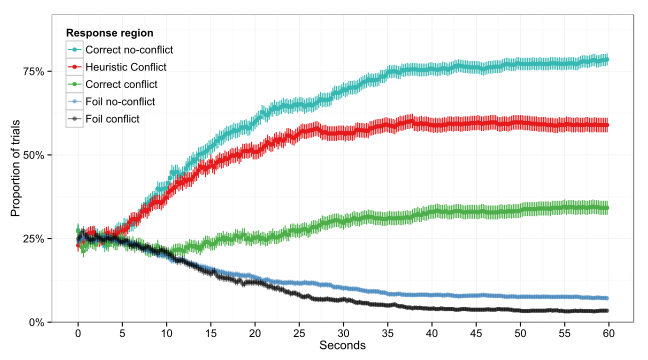
\includegraphics[width=\figurewidth]{imgs/exp6-all.pdf}
  \caption[Proportion of mouse cursors each region of the screen over time, Experiment 6.]{
    \label{fig:exp6-all}
    Proportion of mouse cursors in the region of the screen 
    corresponding to each response options, over time, 
    for conflict and no-conflict problems.    
  }
\end{figure}

\begin{figure}[bp]
  \centering
  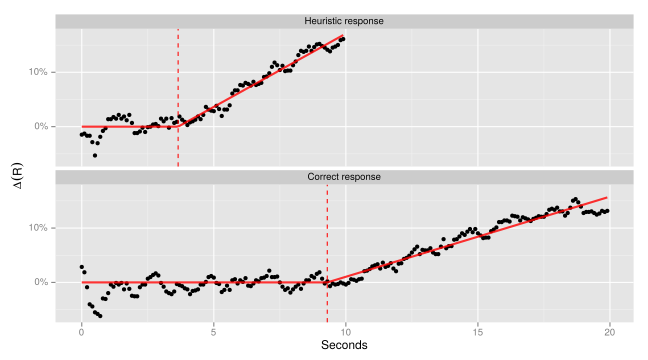
\includegraphics[width=\figurewidth]{imgs/exp6_changepoint.pdf}
  \caption[Change point analysis, Experiment 6.]{
    \label{fig:exp6_changepoint}
    Top: $\Delta (Heuristic)$, the difference between
    the probability of the cursor being in the region of the heuristic option
    and the probability of being in the region of a foil option.\\
    Bottom: $\Delta (Correct)$, the difference between
    the probability of being in the region of the correct option,
    and of being in the region of a foil option.
    Solid red lines show non-linear regression fits.
    Dashed vertical lines show change points,
    after which participants began to be drawn towards the option in question.
  }
\end{figure}

\subsubsection{Bayesian Change Point Analysis}

Inspecting Figure~\ref{fig:exp6-all},
participants are initially equally likely
to move toward each of the four response options
on conflict trials, doing so 25\% of the time.
This is the case until some time before 5 seconds,
at which point participants become more likely
to be in the region of the heuristic option
than the correct option, or either of the foils,
reflecting the point at which processes driving participants
towards the heuristic response exert their influence.
Similarly participants were equally likely to be
in the region of the correct option as the foils
until around 10 seconds,
and after this point more likely to be in the region of the correct option,
indicating that participants begin to be drawn towards the correct option
from this time.

Of course, visual inspection of these curves
is not a particularly accurate means of revealing
\emph{when} participants begin to be drawn towards each response option.
To formally estimate the times at which
participants began to move towards each response,
I calculated, across each 40 msec,
$\Delta (Heuristic)$: the difference between the average probability
of the cursor being in the region of the heuristic option
and the probability of being in the region of either foil option, as well as
$\Delta (Correct)$: the difference between the average probability
of being in the region of the correct option
and of being in the region of the foil option.
This yielded two series of values (Figure~\ref{fig:exp6_changepoint})
that were close to $0$ until participants
began to be drawn towards the response in question,
and increased over time after that point.

I modelled these series using a non-linear regression model
of the form

\begin{equation*}
  \Delta (R) =
  \begin{cases}%
    0          & \text{if}\ t\ <\ \tau_{R} \\
    \beta * (t-\tau_{R})  & \text{otherwise}%
  \end{cases}
\end{equation*}

where $t$ is the time in seconds,
$\tau_{R}$  is the point at which
participants begin to be drawn towards response $R$,
and $\beta$ is the slope of the regression line
after time $\tau_{R}$.

Modelling $\Delta (Heuristic)$, I analysed the first 10 seconds of each trial,
and set a uniform prior on the value of $\tau_{Heuristic}$ between 0 and 10 seconds
(i.e. that participants were equally likely to start being drawn
towards the heuristic response any time between 0 and 10 seconds into a trial).
Modelling $\Delta (Correct)$, I analysed the first 20 second,
and again set a uniform prior on $\tau_{Correct}$ between 0 and 20 seconds.
In both cases, I set an uninformative normal prior
with mean 0 and SD 1 on the slope, $\beta$.

Figure~\ref{fig:exp6_changepoint} shows the fitted regression models,
and Table~\ref{tbl:exp6_changepoint} shows the posterior estimates for the parameters.
The posteriors for the $\tau$ parameters represent
estimates of the point at which participants began to be drawn to each response.
The median posterior estimate for $\tau_{Heuristic}$ was
3.65 seconds (95\% credible interval [3.36, 3.93 seconds]),
and the estimate for $\tau_{Correct}$ was
9.30 seconds (95\% credible interval [8.86, 9.64 seconds]).
The $\beta$ parameters reflect how quickly
the proportion of participants in the region of each option increased after time $\tau$.
The estimate for $\beta_{Heuristic}$
(median 0.027, or a 2.7\% increase per second,
95\% credible interval [2.5\%, 2.9\%])
was almost twice as large as that for $\beta_{Correct}$
(median 0.015, or a 1.5\% increase per second,
95\% credible interval [1.4\%, 1.6\%]).
To summarise, participants began to be drawn towards
the heuristic option from 3.6 seconds,
and towards the correct option from 9.3 seconds.
After these onsets of attraction,
there was a greater increase in the proportion of trials
where the cursor was in the region of the heuristic option (2.7\% per second)
than in the proportion of trials
where it was in the region of the correct option (1.5\% per second).


\begin{table}
  \centering
  \caption[Bayesian change point analysis, Experiment 6.]{
    Posterior estimates from the change point analysis.
    Participants began to be drawn towards the heuristic option
    from 3.65 seconds, and the correct option from 9.30 seconds.
    \label{tbl:exp6_changepoint}
  }
  \begin{tabular}{lrrr}
    \toprule
    Parameter           & Median & 2.5\% & 97.5\%\\
    \midrule
    $\tau_{Heuristic}$  & 3.65  & 3.36 & 3.93\\
    $\tau_{Correct}$    & 9.30  & 8.86 & 9.64\\
    \midrule
    $\beta_{Heuristic}$ & 0.027  & 0.025 & 0.029\\
    $\beta_{Correct}$   & 0.015  & 0.014 & 0.016\\
    \bottomrule
  \end{tabular}
\end{table}



\subsubsection{Growth curve modelling}

\begin{figure}[ht]
  \centering
  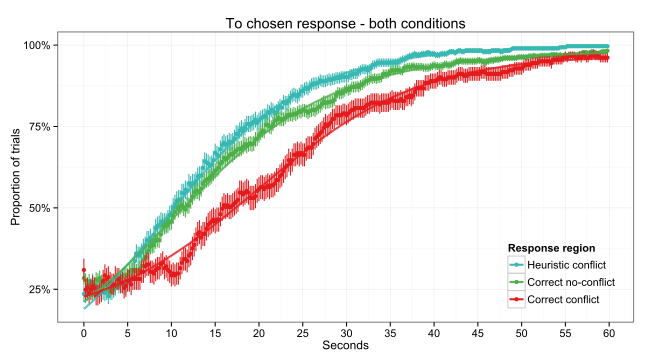
\includegraphics[width=\figurewidth]{imgs/exp6-all-to-chosen.pdf}
  \caption[Proportion of cursor in region of chosen response option, Experiment 6.]{
    \label{fig:exp6-all-to-chosen}
    Proportion of mouse cursors in the region of
    the response option which was ultimately selected on that trial.    
  }
\end{figure}

This time course data also allows us to
supplement the response time analyses reported above
by looking at the speed at which participants moved the mouse cursor to
the region of the response option they eventually did select.
Figure 4 shows this measure for correct responses to no-conflict problems,
and for both heuristic and correct responses to conflict problems.
The curve for each response region over time
was modelled using third-order polynomial logistic regression models
\citep[or growth curves; see][]{Mirman2014},
such that the log odds of the cursor being in that region were given as
$\alpha + \beta_1 t + \beta_2 t^2 + \beta_3 t^3$.
Natural polynomials were used,
meaning that the intercept corresponded to the log odds at 0 seconds,
the linear term to the simple change over time,
and the quadratic and cubic terms to higher-order 'wiggles' later in the time course.%
\footnote{
  One disadvantage of using these natural polynomial terms
  is that they are by definition correlated,
  and so the model suffers from mild multicollinearity,
  which leads to some loss of statistical power.
  However, as the alternative, orthogonal polynomial terms
  would be difficult to interpret individually,
  I believe this approach lends itself
  to a clearer description of the data.
  }

To test for a significant difference between two curves,
a null model, in which the  weights were the same for each curve,
was compared with a full model, in which there were different  weights for each curve.
Chi-squared tests were used to compare the deviance of each model,
with degrees of freedom corresponding to the number of  parameters added in the full model.
Note that $\alpha$, the intercept, was not allowed to vary between curves.
Finally, a random effect for the linear time term was included for each participant,
to allow for individual variability in
how quickly each participant moved towards a response in general.
Random effects on other terms, by participant, or by problem, were considered,
but led to convergence issues, and so only this term,
which was found to account for the most variance, was included.

Mirroring the response time analyses, and as predicted by all dual process accounts,
participant were faster to move towards
the heuristic response option when selecting it
than the correct option for conflict problems
($\chi^2$ = 4515.7, DF = 3, p < .0001),
with the curves differing significantly on the linear, quadratic, and cubic terms
(z's > 5, p's < .0001; see Figure~\ref{fig:exp6-all-to-chosen}).
Again consistent with the response time analyses,
and contrary to previous findings supportive of the intuitive logic model,
participants were faster to move towards the heuristic response on conflict problems
then to move towards the correct response on no-conflict problems
($\chi^2$, DF = 3, p < .0001).
This effect was mainly driven by a significant difference
on the linear term between the curves (z = 2.352, p = .0187).

Most dual process theories, including default-interventionist,
parallel-competitive, and intuitive logic accounts,
would predict that participants should be
drawn towards the heuristic option
on trials where they ultimately give the correct response.
In order to test for this attraction,
I compared the probability over time of
the cursor being in the region of the heuristic option
with the average probability of it being in the region of
either foil option on those trials (Figure~\ref{fig:exp6-correct-not-chosen}).
A higher probability of being in the region of the heuristic option
than the foils constitutes evidence of an attraction towards that heuristic response.
Visual inspection of Figure~\ref{fig:exp6-correct-not-chosen} shows that
this is the case from approximately 10 seconds onwards.
Again, third order polynomial regression models were fit to this data,
which showed that the difference between the curves was statistically significant
($\chi^2$ = 428.2, DF = 3, p < .0001),
with significant differences on the linear, quadratic, and cubic terms
(z's > 2.1, p's < .05).
Therefore, when selecting the correct response,
participants were more drawn to the heuristic option than to the foils,
as predicted both by default-interventionist
and parallel-competitive or intuitive logic accounts.

\begin{figure}[pt]
  \centering
  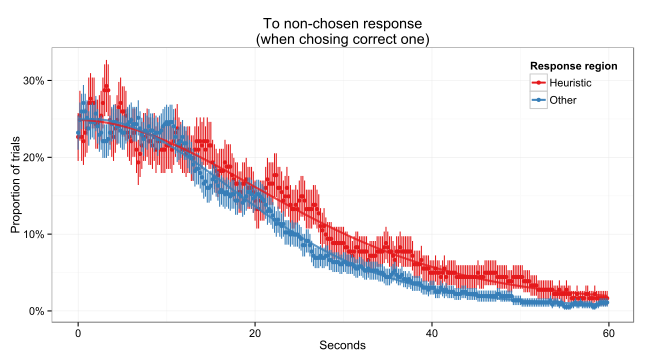
\includegraphics[width=\figurewidth]{imgs/exp6-correct-not-chosen.pdf}
  \caption[Proportion of cursor in region of other response options
  when correct response was given, Experiment 6.]{
    \label{fig:exp6-correct-not-chosen}
    Proportion of trials in the region of each option, over time,
    for trials in which the correct option was eventually chosen,
    for conflict problems.
    Error bars show standard error of measurement.
    Lines show fitted polynomial regression curves.
    Participants were more likely to be in the region of the heuristic response from around 10 seconds onwards.
  }
\end{figure}

\begin{figure}[pb]
  \centering
  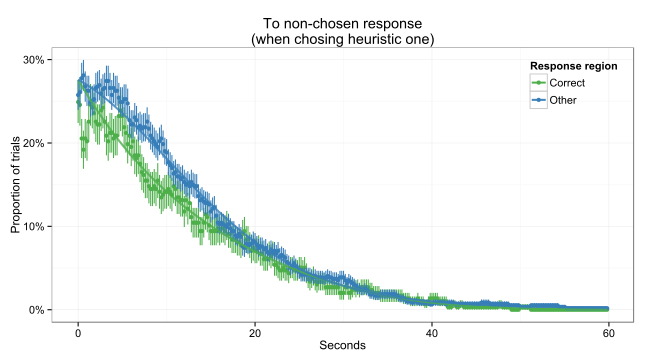
\includegraphics[width=\figurewidth]{imgs/exp6-heuristic-not-chosen.pdf}
  \caption[Proportion of cursor in region of other response options
  when heuristic response was given, Experiment 6.]{
    \label{fig:exp6-heuristic-not-chosen}
    Proportion of trials in the region of each option, over time,
    for trials in which the intuitive option was eventually chosen,
    for conflict problems.
    Participants were less or equally likely to be
    in the region of the correct option than a foil throughout.
  }
\end{figure}


A more interesting comparison is between
the attraction towards the correct response option,
and that towards the foil options,
on conflict trials where the heuristic response is given.
According to the default-interventionist account,
Type 2 processes have not become engaged at this point,
and so the correct response option should not be
any more attractive than the foil options.
According to the parallel-competitive account,
on the other hand, both Type 1 and Type 2 processes
should be engaged on such trials,
and so participants should be drawn towards
giving the response cued by Type 2 processes
(that is, the correct response).
Either result could be consistent with the intuitive logic theory,
depending on the mechanism by which conflict is actually detected.
If conflict detection occurs because
Type 1 processes simultaneously cue both the correct and heuristic responses,
then attraction towards the correct response option should be seen here.
Conversely, if conflict is detected
without Type 1 processes actually producing the correct response,
then the intuitive logic theory,
like the classic default-interventionist account,
would predict no attraction towards the correct response option here.
Of course, no conflict would be predicted by a selective theory.

Figure~\ref{fig:exp6-heuristic-not-chosen} shows that,
contrary to the prediction of the parallel-competitive
and intuitive logic accounts,
participants are not more likely to move towards the correct response option
than either of the foils before giving the heuristic response.
Participants were in fact less likely
to be in the region of the correct option than the foils.
The polynomial regression model showed that
the difference between the curves shown is again significant
($\chi^2$ = 208.0, DF = 3, p < .0001),
with significant differences between the curves on the
linear, quadratic, and cubic terms (z's > 9, p's < .0001).
This result indicates that the correct responses were on average
actually less attractive than the foils.
This is perhaps unsurprising,
given that part of the difficulty of the CRT
lies in the failure of intuition to support the correct response.

%% Finally, once again following previous tests of
%% the intuitive logic theory \citep[e.g.][]{Mevel2014},
%% I repeated the time course analyses reported above for both the
%% ``majority heuristic'' and ``minority heuristic'' participants.
%% The plots for these analyses are shown in Appendix~\ref{appendix:exp6_participants},
%% and reveal that my main findings hold for
%% both sets of participants.
%% \aside{This bit is tricky, especially after the reviews.
%%   Talk about by-item differences here?
%%   Eye balling them, there really is no difference for the bat and ball problems,
%%   but maybe I could test this?}
%% Appendix~\ref{appendix:exp6_items} shows the same analyses
%% plotted separately for each of the eight CRT problems.
%% Again, the results described broadly hold true across all items.
%% However, the bat-and-ball question
%% can be seen to differ slightly from the others
%% in some of the analyses here.
%% I explore this discrepancy in Appendix~\ref{appendix:exp6_items_model}.

\FloatBarrier


\section{Discussion}

These results are broadly consistent with
a default-interventionist dual process theory
\citep{Evans2006,Kahneman2005}.
On problems with an incorrect but intuitively appealing heuristic response,
this response was given more quickly,
and with less evidence of conflict,
than the correct response.
Participants began to systematically move the mouse cursor
to the region of the heuristic response option within approximately 5 seconds,
compared to 10 seconds for movements to the correct response option,
and this trend was evident both when analysing all trials,
and trials in which the response in question was given.
This also appears to be true of both biased and unbiased participants. 

When participants did give the correct response on these conflict problems,
they spent more time in the region of the heuristic response option
than either of the foil options before doing so ---
a finding consistent with default-interventionist,
parallel-competitive, and intuitive logic accounts,
suggesting that these participants considered the heuristic response
before they reached the correct one.
This finding is also consistent with modelling work
\citep{Bockenholt2012,Campitelli2013},
and individual differences studies \citep{Liberali2012}
which have shown that inhibition of the heuristic response
is an important predictor of accuracy on the CRT.
However, contrary to the prediction made from
a parallel-competitive dual process theory
\citep{Sloman1996,Sloman2014}
or by the intuitive logic account
\citep{DeNeys2014a,DeNeys2012,Handley2015}
on trials where the heuristic response was given
participants were no more likely to place the cursor
in the region of the correct response option than either foil option.

These results also have implications for the logical intuitions theory
\citep{DeNeys2012,DeNeys2014a}.
First, a number of previous studies using simpler reasoning tasks
have found that heuristic responses to conflict problems take longer
than correct responses to no-conflict problems,
despite both being cued by Type 1 processes
\citep{DeNeys2008,Stupple2008}.
To my knowledge, the current study is the first to report response times
for conflict and no-conflict versions of the CRT,
and although this analysis was not the main focus of the this experiment,
I found no such effect.
In fact, when analysing participants speed of movement
to the response option they ultimately selected, a more sensitive measure,
I found the opposite effect,
with participants faster to move to the heuristic option under conflict
than the correct option for no-conflict problems
on trials where these responses were given.
All of these findings were true for both
participants who gave the heuristic response to most conflict problems,
and those who did not.
Thus, unlike a number of studies using simpler reasoning problems,
I found no evidence that participants were slower
to give intuitively-cued responses which were wrong
than intuitively-cued responses which were right.

Secondly, as discussed above, I found no evidence of
an attraction towards the correct response option
on conflict problems where the heuristic response was given.
This suggests that Type 1 processes did not simultaneously
cue both responses on such trials.
This result is not, however, totally inconsistent with the logical intuitions theory.
Previously, I differentiated between
a dual process conflict monitoring account \citep{DeNeys2008,DeNeys2008a},
that proposes that we detect when our reasoning is biased,
and a fully-fledged intuitive logic theory \citep{DeNeys2012,DeNeys2014a,Handley2015},
where this conflict detection is the result
of Type 1 processes simultaneously cuing
both the correct and the heuristic response.
These results would appear to contradict the latter account,
%% \citep{DeNeys2012,Handley2015,Pennycook2015,DeNeys2014a}
whereby Type 1 processes cue both the heuristic response (``10p'')
and the correct response (``5p'') at the same time
for the bat-and-ball problem and other CRT items.
They do not, however, rule out the possibility that
participants experience uncertainty \citep{DeNeys2013a},
or a feeling of wrongness \citep{Gangemi2015}
while solving these conflict problems.
If this is the case, further work is needed to reveal how this feeling comes about.

At this point, I would like to note again that,
\citet{DeNeys2013a} and \citep{Gangemi2015} notwithstanding,
previous evidence for the intuitive logic theory has come from simpler experiments,
such as simple syllogistic reasoning \citep{Morsanyi2012}
and forced-choice base rate neglect \citep{DeNeys2008} paradigms.
The operations required to reach the correct answer to these CRT problems
are considerably more complex than those needed to evaluate a simple syllogism,
or apply basic statistical principles.
Therefore, while I do not find evidence that Type 1 processes
automatically generate correct responses on the CRT,
this does not rule out the possibility that they can
generate correct responses on these simpler tasks.
For instance, it has been demonstrated that participants
report ``liking'' syllogisms which are logically valid
more than those which are invalid,
even when not asked to evaluate their logical status \citep{Morsanyi2012},
but also that this effect only holds for simpler logical forms
\citep[see also \citealp{Handley2015}]{Klauer2013}.
Indeed, \citet{DeNeys2012},
when proposing the intuitive logic account
raised the possibility that it
may not apply to all problems.
%% With this in mind, it is worth considering if
%% the reductions in confidence for conflict problems reported by
%% \citet{DeNeys2013} and \citet{Gangemi2015} can be explained
%% without recourse to logical intuitions.
%% One possibility is that participants were engaged in \emph{rationalisation}
%% \citep{Ball2003,Evans2006,Pennycook2015}.
%% That is, while Type 1 processes cued initial responses,
%% participants in both conditions may engage shallow Type 2 processes
%% to attempt to verify them.
%% For no-conflict problems, participants can easily verify
%% that their intuitive response is correct,
%% and so give it with confidence.
%% For conflict problems, on the other hand,
%% their initial responses would be incorrect,
%% and so they would not be able to validate them.
%% Some participants would give these unvalidated responses,
%% but lack confidence in doing so,
%% while others would engage further Type 2 processes to produce the correct response.
%% Crucially, such an account would not require that
%% participants implicitly detect the error in their initial responses.
%% This account should also be testable in future.
%% If the reduction in confidence is the product of an implicit detection of conflict,
%% it should occur early in the reasoning processes.
%% Alternatively, if it is the product of
%% an inability to explicitly validate an intuitive response,
%% the reduction in confidence should occur later,
%% after these shallow Type 2 processes have been engaged.
%% I would stress at this point, however,
%% that I do not dispute the validity of the intuitive logic theory more broadly here,
%% but rather question if it applies equally to complex logical tasks as to simple ones.

One might argue that the absence of evidence for either
the parallel-competitive or intuitive logical theories here
do not reflect evidence against these accounts,
but rather the inability of this paradigm to reveal
the effects predicted  by these accounts.
It may be the case, according to this line of reasoning,
that participants are drawn towards the correct option
on trials where they give the heuristic response,
or that participants are more conflicted
when their heuristic responses are wrong than when they are right,
but that I was unable to detect these mental states using this new paradigm.
While I cannot completely rule out this possibility,
I believe two factors go against such an interpretation.
First, this paradigm does reveal effects,
such as attraction towards the heuristic option before giving the correct response,
consistent with the default-interventionist model.
Second, for the two comparisons above, rather than finding no effect,
I found significant effects in the opposite direction
to those predicted by parallel-competitive and intuitive logic accounts.

Additionally, there is extensive evidence that
even subtle, implicit cognitive processes
influence motor output in detectable ways
\citep{Tucker2004,Xiao2014,Miles2010,Bargh2006}.
Therefore, if participants do experience conflict,
but this conflict does not influence their motor output,
then this raises the question of
what  mechanism produces this conflict
while not influencing motor output.
I return to this issue in Chapter 7.
Finally, I would note again that these results
should be interpreted as
constraining the intuitive logic account,
rather than falsifying it.

Of course, all of the above assumes a dual process interpretation of the CRT,
as most treatments of the task do.
Even in accounts which focus instead on dispositional factors
\citep{Campitelli2013,Campitelli2010a},
it is acknowledged that responding correctly typically requires
the inhibition of the heuristic response.
While I am unaware of any accounts of the CRT
which do not rely on such an inhibition,
I cannot rule out the possibility of such explanations being offered in future.
The current results, however, provide an additional constraint to such accounts,
in that they should predict not only observed choices,
but also the patterns at the process level reported here.

As a side note, it may be noted that it is unusual
to present the CRT as a multiple-choice test,
and that this may affect the processes engaged during this experiment.
However, multiple-choice versions for the test have been previously reported
by \citet{morsanyi2014mathematical}, \citet[][Experiment 3]{Primi2015},
and \citet[][Experiment 2]{Gangemi2015},
without any clear effect on participants’ responses.


Finally, since its introduction in 2005, the CRT has been hugely popular
as a measure of individual differences in thinking,
despite only limited evidence as to what underlies performance on the task.
These results go some way towards filling this gap,
and suggest that responding correctly
does require the activation of otherwise dormant Type 2 processes
to override incorrect intuitions.
Future work might address the relationship between
conflict on this task and individual differences.
\citet{Stanovich2008} proposed that normative decision making requires
(1) awareness of the limitations of intuition;
(2) desire to overcome those limitations;
(3) inhibition of the intuitive response and
(4) ability to generate the correct response.
Each of these requirements is a distinct reason for
failure to produce the correct response on the CRT,
and each should produce a distinctive pattern in mouse cursor movement data.

To conclude, I recorded participants' mouse cursor movements
over a considerable period of time
while they reasoned about CRT problems.
Trends in these movements were consistent with
a default-interventionist dual process theory of reasoning,
where participants are initially drawn towards heuristic responses only,
but in some cases engage further effortful processing to find correct solutions.
I did not find evidence that participants were
drawn to correct responses on trials where these responses were not actually given,
inconsistent with a parallel-competitive dual process account.
Finally, contrary to previous work using simpler reasoning tasks,
and confidence ratings collected on the CRT,
I found no evidence that participants were conflicted
when giving incorrect heuristic responses. 




\begin{appendices}
  %% \setcounter{secnumdepth}{0}
  \appendixpage
  \graphicspath{{./../Appendices/}}

  \chapter{CRT Reasoning Problems from Experiment 6}\label{appendix:exp6_stimuli}
  \begin{center}
  \singlespacing
  \begin{longtable}{llrrlrr}
    \caption[]{
      Stimuli used in Experiment 6.
      Items 1--3 were adapted from \citet{Frederick2005}.
      Items 4--8 were adapted from \citet{Primi2015}.
      \emph{Note.} Percentages in parentheses show the proportion of participants who gave each response.
    }\\
    \toprule
    & \multicolumn{3}{l}{Conflict} & \multicolumn{3}{l}{No-conflict} \\
    \midrule
    \endfirsthead
    \toprule
    & \multicolumn{3}{l}{Conflict} & \multicolumn{3}{l}{No-conflict} \\
    \midrule
    \endhead

    \bottomrule
    \endfoot

    \bottomrule\bottomrule
    \endlastfoot

    1 &
    \multicolumn{3}{ p{.4\textwidth} }{
      A bat and a ball together costs £1.10.
      A bat costs £1 more than a ball.
      How~much~does~a~ball~cost?}
    & \multicolumn{3}{ p{.4\textwidth} }{
      A bat and a ball together costs £1.05.
      A bat costs £1.
      How much does a ball cost?
    } \\*
    \\*
    & Correct response:   & 5p   &(15\%) &  Correct response:  & 5p & (97\%)\\*
    & Heuristic response: & 10p   &(83\%) &  Foil response:     & 10p & (0\%)\\*
    & Foil response:      & 15p   &(0\%)  &  Foil response:    & 15p & (1\%)\\*
    & Foil response:      & 90p   &(2\%)  &  Foil response:    & 90p & (1\%)\\
    \midrule

    2 &
    \multicolumn{3}{ p{.4\textwidth} }{
      It takes 5 machines 5 minutes to make 5 
      widgets. How many minutes would it take 100
      machines to make 100 widgets?}
    & \multicolumn{3}{ p{.4\textwidth} }{
      It takes a machine 5 minutes to make 5 
      widgets. How many minutes would it take the
      machines to make 100 widgets?
    } \\*
    \\*
    & Correct response:   & 5   &(24\%) &  Correct response:  & 100 & (83\%)\\*
    & Heuristic response: & 100   &(69\%) &  Foil response:     & 5 & (2\%)\\*
    & Foil response:      & 50   &(4\%)  &  Foil response:    & 50 & (13\%)\\*
    & Foil response:      & 10   &(3\%)  &  Foil response:    & 10 & (2\%)\\
    \midrule

    3 &
    \multicolumn{3}{ p{.4\textwidth} }{
      In a lake, there is a patch of lily pads.
      Every day, the patch doubles in size.
      If it takes 48 days for the patch to cover
      the entire lake, how many days would it take
      for the patch to cover half of the lake?}
    & \multicolumn{3}{ p{.4\textwidth} }{
      In a lake, there is a patch of lily pads.
      Every day, the patch grows by 10m².
      If it takes 48 days for the patch to cover
      the 150m², how many days would it take
      for the patch to cover 140m²?
    } \\*
    \\*
    & Correct response:   & 47   &(25\%) &  Correct response:  & 47 & (79\%)\\*
    & Heuristic response: & 24   &(59\%) &  Foil response:     & 24 & (17\%)\\*
    & Foil response:      & 12   &(15\%)  &  Foil response:    & 12 & (4\%)\\*
    & Foil response:      & 2   &(2\%)  &  Foil response:    & 2 & (0\%)\\
    \bottomrule

    4 &
    \multicolumn{3}{ p{.4\textwidth} }{
      If you flipped a fair coin twice, what is
      the probability that it would land
      'Heads' at least once?}
    & \multicolumn{3}{ p{.4\textwidth} }{
      If you flipped a fair coin twice, what is
      the probability that it would land
      'Heads' exactly once?
    } \\*
    \\*
    & Correct response:   & 75\%   &(4\%) &  Correct response:  & 25\% & (68\%)\\*
    & Heuristic response: & 50\%   &(84\%) &  Foil response:     & 50\% & (26\%)\\*
    & Foil response:      & 25\%   &(11\%)  &  Foil response:    & 75\% & (6\%)\\*
    & Foil response:      & 100\%   &(1\%)  &  Foil response:    & 100\% & (0\%)\\
    \midrule

    5 &
    \multicolumn{3}{ p{.4\textwidth} }{
      If 3 elves can wrap 3 toys in
      1 hour, how many elves are needed
      to wrap 6 toys in 2 hours?}
    & \multicolumn{3}{ p{.4\textwidth} }{
      If 3 elves can wrap 3 toys in
      1 hour, how many toys could 6 elves
      wrap in half an hour?
    } \\*
    \\*
    & Correct response:   & 3   &(73\%) &  Correct response:  & 3 & (71\%)\\*
    & Heuristic response: & 6   &(22\%) &  Foil response:     & 6 & (20\%)\\*
    & Foil response:      & 1   &(2\%)  &  Foil response:    & 1 & (1\%)\\*
    & Foil response:      & 12   &(4\%)  &  Foil response:    & 12 & (8\%)\\*
    \midrule

    6 &
    \multicolumn{3}{ p{.4\textwidth} }{
      Ellen and Kim are running around a track.
      They run equally fast but Ellen started later.
      When Ellen has run 5 laps, Kim has run 10 laps.
      When Ellen has run 10 laps, how many has Kim run?}
    & \multicolumn{3}{ p{.4\textwidth} }{
      Ellen and Kim are running around a track.
      They started at the same time,
      but Kim is twice as fast as Ellen.
      When Ellen has run 5 laps, Kim has run 10 laps.
      When Ellen has run 10 laps, how many has Kim run?
    } \\*
    \\*
    & Correct response:   & 15   &(73\%) &  Correct response:  & 20 & (98\%)\\*
    & Heuristic response: & 20   &(27\%) &  Foil response:     & 15 & (2\%)\\*
    & Foil response:      & 5   &(0\%)  &  Foil response:    & 5 & (0\%)\\*
    & Foil response:      & 19   &(0\%)  &  Foil response:    & 19 & (0\%)\\
    \midrule

    7 &
    \multicolumn{3}{ p{.4\textwidth} }{
      Jerry received both the 15th highest and
      the 15th lowest mark in the class. How many
      students are there in the class?}
    & \multicolumn{3}{ p{.4\textwidth} }{
      Jerry received both the 2nd highest and
      the 2nd lowest mark in the class. How many
      students are there in the class?
    } \\*
    \\*
    & Correct response:   & 29   &(26\%) &  Correct response:  & 3 & (79\%)\\*
    & Heuristic response: & 30   &(72\%) &  Foil response:     & 2 & (13\%)\\*
    & Foil response:      & 40   &(2\%)  &  Foil response:    & 5 & (8\%)\\*
    & Foil response:      & 5   &(0\%)  &  Foil response:    & 10 & (0\%)\\
    \midrule

    8 &
    \multicolumn{3}{ p{.4\textwidth} }{
      In an athletics team tall members tend to win
      three times as many medals than short members.
      This year the team has won 60 medals so far.
      How many of these have been won by short athletes?}
    & \multicolumn{3}{ p{.4\textwidth} }{
      In an athletics team tall members tend to win
      twice as many medals than short members.
      This year the team has won 60 medals so far.
      How many of these have been won by short athletes?
    } \\*
    \\*
    & Correct response:   & 15   &(44\%) &  Correct response:  & 20 & (58\%)\\*
    & Heuristic response: & 20   &(52\%) &  Foil response:     & 15 & (12\%)\\*
    & Foil response:      & 30   &(1\%)  &  Foil response:    & 30 & (27\%)\\*
    & Foil response:      & 50   &(3\%)  &  Foil response:    & 50 & (4\%)\\
  \end{longtable}
\end{center}

%% \begin{table}[!h]
%%   \centering
%%   \caption[]{
%%     Stimuli used in Experiment 6.
%%     Items 1--3 were adapted from \citet{Frederick2005}.
%%     Items 4--8 were adapted from \citet{Primi2015}.
%%     \emph{Note.} Percentages in parentheses show the proportion of participants who gave each response.
%%   }
%%   \singlespacing
%%   \footnotesize
%%   \begin{tabular}{llrrlrr}
%%     \toprule
%%     & \multicolumn{3}{l}{Conflict} & \multicolumn{3}{l}{No-conflict} \\
%%     \midrule

%%     %% \parbox[b]{2mm}{\multirow{6}{*}{\rotatebox[origin=c]{90}{1. Bat-and-ball}}} &
%%     1 &
%%     \multicolumn{3}{ p{.4\textwidth} }{
%%       A bat and a ball together costs £1.10.
%%       A bat costs £1 more than a ball.
%%       How~much~does~a~ball~cost?}
%%     & \multicolumn{3}{ p{.4\textwidth} }{
%%       A bat and a ball together costs £1.05.
%%       A bat costs £1.
%%       How much does a ball cost?
%%     } \\
%%     \\
%%     & Correct response:   & 5p   &(15\%) &  Correct response:  & 5p & (97\%)\\*
%%     & Heuristic response: & 10p   &(83\%) &  Foil response:     & 10p & (0\%)\\*
%%     & Foil response:      & 15p   &(0\%)  &  Foil response:    & 15p & (1\%)\\*
%%     & Foil response:      & 90p   &(2\%)  &  Foil response:    & 90p & (1\%)\\*
%%     \midrule

%%     2 &
%%     \multicolumn{3}{ p{.4\textwidth} }{
%%       It takes 5 machines 5 minutes to make 5 
%%       widgets. How many minutes would it take 100
%%       machines to make 100 widgets?}
%%     & \multicolumn{3}{ p{.4\textwidth} }{
%%       It takes a machine 5 minutes to make 5 
%%       widgets. How many minutes would it take the
%%       machines to make 100 widgets?
%%     } \\
%%     \\
%%     & Correct response:   & 5   &(24\%) &  Correct response:  & 100 & (83\%)\\*
%%     & Heuristic response: & 100   &(69\%) &  Foil response:     & 5 & (2\%)\\*
%%     & Foil response:      & 50   &(4\%)  &  Foil response:    & 50 & (13\%)\\*
%%     & Foil response:      & 10   &(3\%)  &  Foil response:    & 10 & (2\%)\\*
%%     \midrule

%%     3 &
%%     \multicolumn{3}{ p{.4\textwidth} }{
%%       In a lake, there is a patch of lily pads.
%%       Every day, the patch doubles in size.
%%       If it takes 48 days for the patch to cover
%%       the entire lake, how many days would it take
%%       for the patch to cover half of the lake?}
%%     & \multicolumn{3}{ p{.4\textwidth} }{
%%       In a lake, there is a patch of lily pads.
%%       Every day, the patch grows by 10m².
%%       If it takes 48 days for the patch to cover
%%       the 150m², how many days would it take
%%       for the patch to cover 140m²?
%%     } \\
%%     \\
%%     & Correct response:   & 47   &(25\%) &  Correct response:  & 47 & (79\%)\\*
%%     & Heuristic response: & 24   &(59\%) &  Foil response:     & 24 & (17\%)\\*
%%     & Foil response:      & 12   &(15\%)  &  Foil response:    & 12 & (4\%)\\*
%%     & Foil response:      & 2   &(2\%)  &  Foil response:    & 2 & (0\%)\\*
%%     \bottomrule
%%   \end{tabular}
%% \end{table}

%% \begin{table}
%%   \centering
%%   \footnotesize
%%   \begin{tabular}{llrrlrr}
%%     \toprule
%%     & \multicolumn{3}{l}{Conflict} & \multicolumn{3}{l}{No-conflict} \\
%%     \midrule

%%     4 &
%%     \multicolumn{3}{ p{.4\textwidth} }{
%%       If you flipped a fair coin twice, what is
%%       the probability that it would land
%%       'Heads' at least once?}
%%     & \multicolumn{3}{ p{.4\textwidth} }{
%%       If you flipped a fair coin twice, what is
%%       the probability that it would land
%%       'Heads' exactly once?
%%     } \\
%%     \\
%%     & Correct response:   & 75\%   &(4\%) &  Correct response:  & 25\% & (68\%)\\*
%%     & Heuristic response: & 50\%   &(84\%) &  Foil response:     & 50\% & (26\%)\\*
%%     & Foil response:      & 25\%   &(11\%)  &  Foil response:    & 75\% & (6\%)\\*
%%     & Foil response:      & 100\%   &(1\%)  &  Foil response:    & 100\% & (0\%)\\*    
%%     \midrule

%%     5 &
%%     \multicolumn{3}{ p{.4\textwidth} }{
%%       If 3 elves can wrap 3 toys in
%%       1 hour, how many elves are needed
%%       to wrap 6 toys in 2 hours?}
%%     & \multicolumn{3}{ p{.4\textwidth} }{
%%       If 3 elves can wrap 3 toys in
%%       1 hour, how many toys could 6 elves
%%       wrap in half an hour?
%%     } \\
%%     \\
%%     & Correct response:   & 3   &(73\%) &  Correct response:  & 3 & (71\%)\\*
%%     & Heuristic response: & 6   &(22\%) &  Foil response:     & 6 & (20\%)\\*
%%     & Foil response:      & 1   &(2\%)  &  Foil response:    & 1 & (1\%)\\*
%%     & Foil response:      & 12   &(4\%)  &  Foil response:    & 12 & (8\%)\\*
%%     \midrule

%%     6 &
%%     \multicolumn{3}{ p{.4\textwidth} }{
%%       Ellen and Kim are running around a track.
%%       They run equally fast but Ellen started later.
%%       When Ellen has run 5 laps, Kim has run 10 laps.
%%       When Ellen has run 10 laps, how many has Kim run?}
%%     & \multicolumn{3}{ p{.4\textwidth} }{
%%       Ellen and Kim are running around a track.
%%       They started at the same time,
%%       but Kim is twice as fast as Ellen.
%%       When Ellen has run 5 laps, Kim has run 10 laps.
%%       When Ellen has run 10 laps, how many has Kim run?
%%     } \\
%%     \\
%%     & Correct response:   & 15   &(73\%) &  Correct response:  & 20 & (98\%)\\*
%%     & Heuristic response: & 20   &(27\%) &  Foil response:     & 15 & (2\%)\\*
%%     & Foil response:      & 5   &(0\%)  &  Foil response:    & 5 & (0\%)\\*
%%     & Foil response:      & 19   &(0\%)  &  Foil response:    & 19 & (0\%)\\*
%%     \midrule

%%     7 &
%%     \multicolumn{3}{ p{.4\textwidth} }{
%%       Jerry received both the 15th highest and
%%       the 15th lowest mark in the class. How many
%%       students are there in the class?}
%%     & \multicolumn{3}{ p{.4\textwidth} }{
%%       Jerry received both the 2nd highest and
%%       the 2nd lowest mark in the class. How many
%%       students are there in the class?
%%     } \\
%%     \\
%%     & Correct response:   & 29   &(26\%) &  Correct response:  & 3 & (79\%)\\*
%%     & Heuristic response: & 30   &(72\%) &  Foil response:     & 2 & (13\%)\\*
%%     & Foil response:      & 40   &(2\%)  &  Foil response:    & 5 & (8\%)\\*
%%     & Foil response:      & 5   &(0\%)  &  Foil response:    & 10 & (0\%)\\*
%%     \midrule

%%     8 &
%%     \multicolumn{3}{ p{.4\textwidth} }{
%%       In an athletics team tall members tend to win
%%       three times as many medals than short members.
%%       This year the team has won 60 medals so far.
%%       How many of these have been won by short athletes?}
%%     & \multicolumn{3}{ p{.4\textwidth} }{
%%       In an athletics team tall members tend to win
%%       twice as many medals than short members.
%%       This year the team has won 60 medals so far.
%%       How many of these have been won by short athletes?
%%     } \\
%%     \\
%%     & Correct response:   & 15   &(44\%) &  Correct response:  & 20 & (58\%)\\*
%%     & Heuristic response: & 20   &(52\%) &  Foil response:     & 15 & (12\%)\\*
%%     & Foil response:      & 30   &(1\%)  &  Foil response:    & 30 & (27\%)\\*
%%     & Foil response:      & 50   &(3\%)  &  Foil response:    & 50 & (4\%)\\*

%%     \bottomrule
%%   \end{tabular}
%% \end{table}



  \chapter{Individual differences in Experiment 6 time course analyses}
  \label{appendix:exp6_participants}
  
Following previous intuitive logic studies \citep[e.g.][]{Mevel2014}
I calculated the number of heuristic responses given
by each participant on conflict problems, 
and categorised each participant as either
``majority heuristic'' (3 or 4 heuristic responses out of four, 53 participants)
or ``minority heuristic'' (0 to 2 heuristic responses, 75 participants).
In this appendix, I repeat the time course analyses
reported for Experiment 6 separately for each group of participants.
As none of the trends differ qualitatively from the results
reported in Chapter 6 in ways that affect my conclusions,
I do not provide interpretation of each individual figure.


\begin{figure}[h]
  \centering
  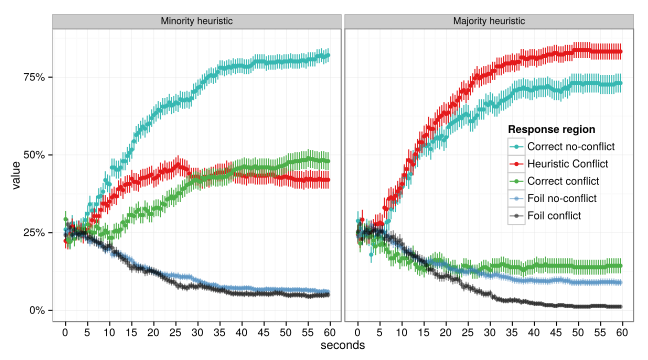
\includegraphics[width=.9\textwidth]{imgs/exp6/all_bias.pdf}
  %% \caption[Proportion of mouse cursors in each responses' region of the screen over time,
  %%   for minority heuristic and majority heuristic particiapants, 
  %%   Experiment 6.]{
  \caption[]{
    Proportion of mouse cursors in the region of the screen 
    corresponding to each response options, over time, 
    for conflict and no-conflict problems,
    separately for minority heuristic and majority heuristic participants
    (see also Figure~\ref{fig:exp6-all}).
  }
\end{figure}

\begin{figure}[h]
  \centering
  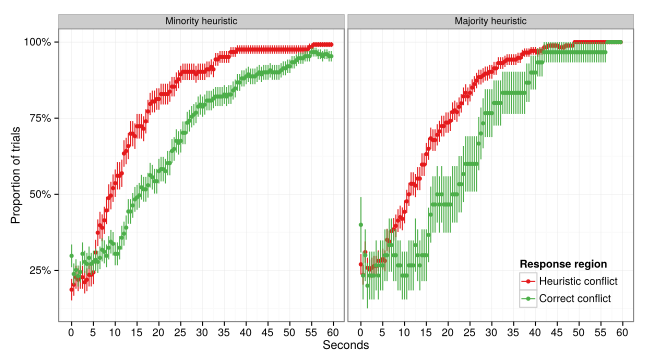
\includegraphics[width=.9\textwidth]{imgs/exp6/conflict-to-chosen_bias.pdf}
  %% \caption[Proportion of cursor in region of chosen response option
  %%   for minority heuristic and majority heuristic particiapants, 
  %%   Experiment 6.]{
  \caption[]{
    Proportion of mouse cursors in the region of
    the response option which was ultimately selected on that trial,
    comparing movements to the heuristic and correct options on conflict problems,
    separately for minority heuristic and majority heuristic participants
    (see also Figure~\ref{fig:exp6-all-to-chosen}).
  }
\end{figure}

\begin{figure}[h]
  \centering
  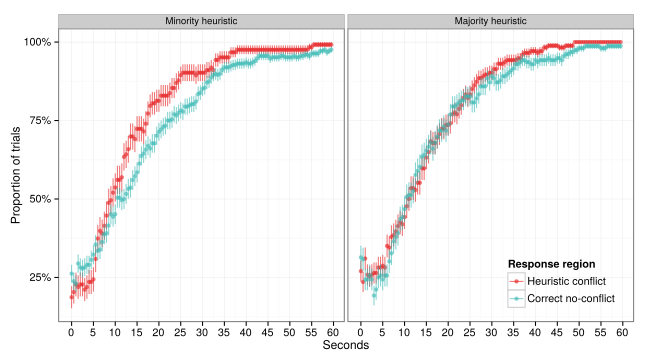
\includegraphics[width=.9\textwidth]{imgs/exp6/intuitive-to-chosen_bias.pdf}
  %% \caption[for minority heuristic and majority heuristic particiapants, 
  %%   Experiment 6.]{
  \caption[]{
    Proportion of mouse cursors in the region of
    the response option which was ultimately selected on that trial,
    comparing movements to the heuristic option conflict problems
    to those to the correct options on no-conflict problems,
    separately for minority heuristic and majority heuristic participants
    (see also Figure~\ref{fig:exp6-all-to-chosen}).
  }
\end{figure}

\begin{figure}[h]
  \centering
  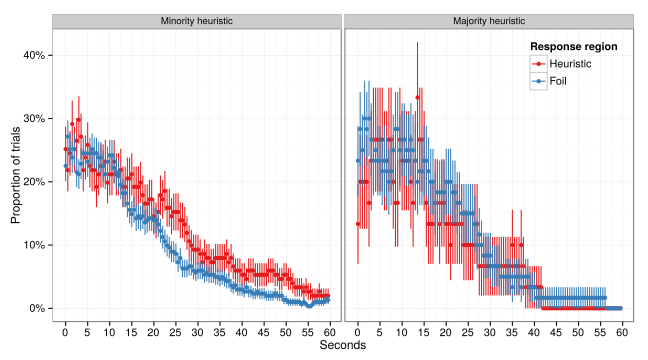
\includegraphics[width=.9\textwidth]{imgs/exp6/correct-not-chosen_bias.pdf}
  %% \caption[Proportion of cursor in region of other response options
  %%   when correct response was given
  %%   for minority heuristic and majority heuristic particiapants, 
  %%   Experiment 6.]{
  \caption[]{   
    Proportion of trials in the region of each option, over time,
    for trials in which the correct option was eventually chosen,
    separately for minority heuristic and majority heuristic participants
    (see also Figure~\ref{fig:exp6-correct-not-chosen}).
    Error bars show standard error of measurement.
  }
\end{figure}

\begin{figure}[h]
  \centering
  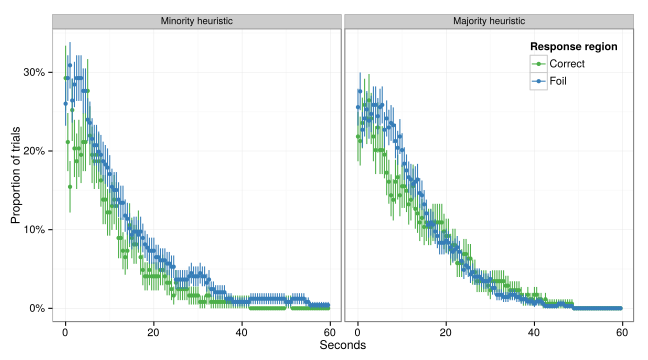
\includegraphics[width=.9\textwidth]{imgs/exp6/heuristic-not-chosen_bias}
  %% \caption[Proportion of cursor in region of other response options
  %%   when heuristic response was given,
  %%   for minority heuristic and majority heuristic particiapants, 
  %%   Experiment 6.]{
  \caption[]{
    Proportion of trials in the region of each option, over time,
    for trials in which the intuitive option was eventually chosen,
    separately for minority heuristic and majority heuristic participants
    (see also Figure~\ref{fig:exp6-heuristic-not-chosen}).
  }
\end{figure}


  \chapter{Differences between problems in Experiment 6 time course analyses}
  \label{appendix:exp6_items}
  
In this Appendix, I plot the time course analyses
for Experiment 6, reported in Chapter 6,
separately for each of the eight CRT problems.
The text of the conflict and no-conflict versions
of the eight items are shown in Appendix~\ref{appendix:exp6_stimuli}.

For clarity, I use labels to refer to each CRT problems.
Therefore, problems 1, 2, and 3 in Appendix~\ref{appendix:exp6_stimuli}
\citep[the original CRT items, from][]{Frederick2005} will be referred to as
the \emph{bat-and-ball}, \emph{widgets}, and \emph{lily pad} problems respectively.
Similarly, problems 5 -- 8, adapted from \citet{Primi2015},
will be referred to the
\emph{coin} (4),
\emph{elves} (5),
\emph{running track} (6),
\emph{grades} (7),
and \emph{athletics team} (8)
problems.


\begin{figure}[h]
  \centering
  \includegraphics[width=.9\textwidth]{imgs/exp6/all_items.pdf}
  %% \caption[Proportion of mouse cursors in each responses' region of the screen over time,
  %% seperately for each problem, Experiment 6.]{
  \caption[]{
    Proportion of mouse cursors in the region of the screen 
    corresponding to each response options, over time, 
    for conflict and no-conflict problems,
    separately for each CRT problem
    (see also Figure~\ref{fig:exp6-all}).
  }
\end{figure}

\begin{figure}[h]
  \centering
  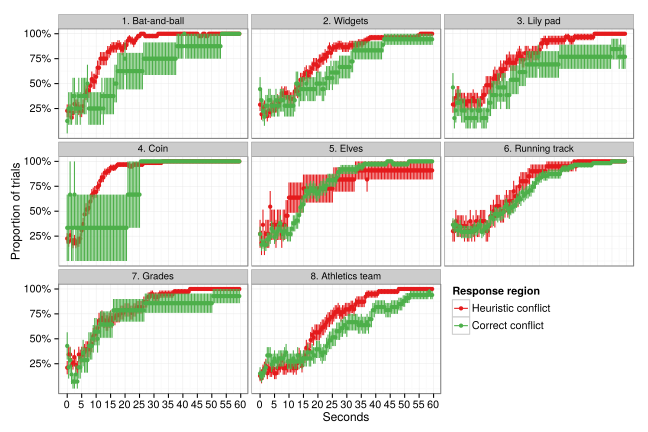
\includegraphics[width=.9\textwidth]{imgs/exp6/conflict-to-chosen_items.pdf}
  %% \caption[Proportion of cursors in region of chosen option,
  %% on conflict problems,
  %% seperately for each problem, Experiment 6.]{
  \caption[]{
    Proportion of mouse cursors in the region of
    the response option which was ultimately selected on that trial,
    comparing movements to the heuristic and correct options on conflict problems,
    separately for each CRT problem
    (see also Figure~\ref{fig:exp6-all-to-chosen}).
  }
\end{figure}

\begin{figure}[h]
  \centering
  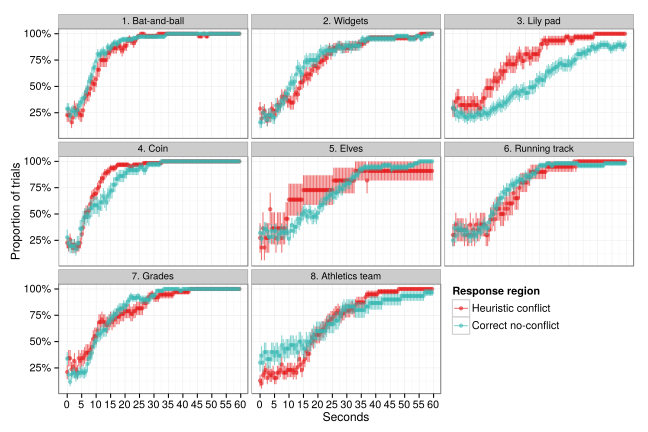
\includegraphics[width=.9\textwidth]{imgs/exp6/intuitive-to-chosen_items.pdf}
  %% \caption[Proportion of cursors in region of chosen option,
  %% for heuristically-cued responses,
  %% seperately for each problem, Experiment 6.]{
  \caption[]{
    Proportion of mouse cursors in the region of
    the response option which was ultimately selected on that trial,
    comparing movements to the heuristic option conflict problems
    to those to the correct options on no-conflict problems,
    separately for each CRT problem
    (see also Figure~\ref{fig:exp6-all-to-chosen}).
    \label{fig:exp6-heuristic-to-chosen-by-item}
  }
\end{figure}


\begin{figure}[h]
  \centering
  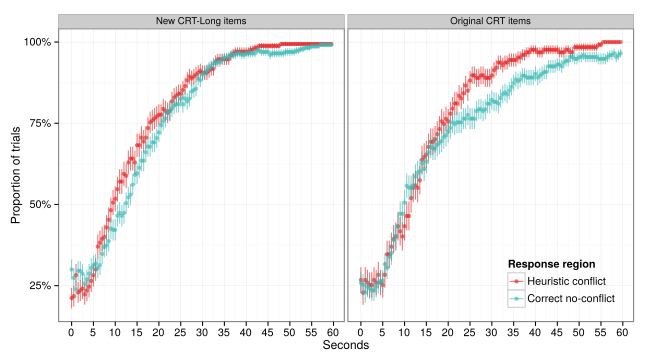
\includegraphics[width=.9\textwidth]{imgs/exp6/intuitive-to-chosen_oldnew.pdf}
  %% \caption[Proportion of cursors in region of chosen option,
  %% for heuristically-cued responses,
  %% seperately for original and extended CRT problems, Experiment 6.]{
  \caption[]{
    Proportion of mouse cursors in the region of
    the response option which was ultimately selected on that trial,
    comparing movements to the heuristic option conflict problems
    to those to the correct options on no-conflict problems,
    separately for the original problems adapted from \citet{Frederick2005},
    and the problems adapted from \citet{Primi2015}
    (see also Figure~\ref{fig:exp6-all-to-chosen}).
  }
\end{figure}




\begin{figure}[h]
  \centering
  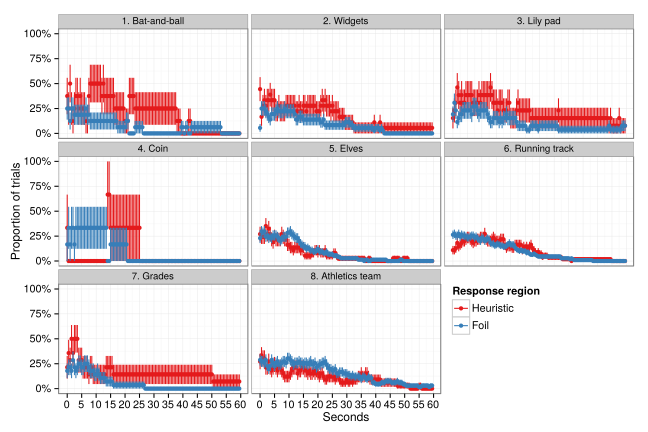
\includegraphics[width=.9\textwidth]{imgs/exp6/correct-not-chosen_items.pdf}
  %% \caption[Proportion of cursor in region of other response options
  %%   when correct response was given,
  %%   seperately for each problem, Experiment 6.]{
  \caption[]{
    Proportion of trials in the region of each option, over time,
    for trials in which the correct option was eventually chosen,
    separately for each CRT problem
    (see also Figure~\ref{fig:exp6-correct-not-chosen}).
    Error bars show standard error of measurement.
  }
\end{figure}

\begin{figure}[h]
  \centering
  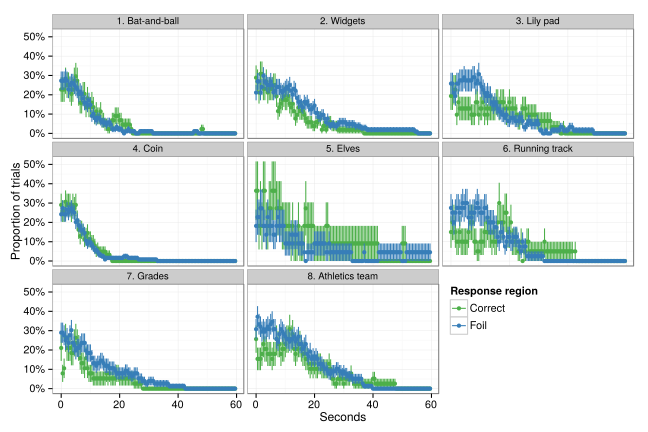
\includegraphics[width=.9\textwidth]{imgs/exp6/heuristic-not-chosen_items.pdf}
  %% \caption[Proportion of cursor in region of other response options
  %%   when heuristic response was given,
  %%   seperately for each problem, Experiment 6.]{
  \caption[]{
    Proportion of trials in the region of each option, over time,
    for trials in which the intuitive option was eventually chosen,
    separately for each CRT problem
    (see also Figure~\ref{fig:exp6-heuristic-not-chosen}).
  }
\end{figure}


\end{appendices}


\bibliography{../references}
\addcontentsline{toc}{chapter}{References}

\end{document}
